\newpage
\chapter*{Capitolo4}
\section{Principi di controllo dell'accesso}
Due definizioni di controllo dell'accesso sono utili per capire la sua portata.
\begin{enumerate}
    \item \textbf{NISTIR 7298} (Glossario dei termini chiave della sicurezza delle informazioni, maggio 2013), definisce il controllo dell'accesso come il processo di concessione o rifiuto di richieste specifiche a:
    
    \begin{itemize}
        \item  Ottenere e utilizzare le informazioni e i relativi servizi di elaborazione delle informazioni
        
        \item  Entrare in specifiche strutture fisiche.
    \end{itemize}
    
    \item \textbf{RFC 4949}, Internet Security Glossary, definisce il controllo dell'accesso come un processo con cui l'uso delle risorse del sistema è regolato secondo una politica di sicurezza è permesso solo alle entità autorizzate (utenti, programmi, processi o altri sistemi) secondo tale politica.
    
Possiamo considerare il controllo degli accessi come un elemento centrale della sicurezza informatica. Gli obiettivi principali della sicurezza informatica sono di impedire agli utenti non autorizzati di accesso alle risorse, impedire agli utenti legittimi di accedere alle risorse in modo non in modo non autorizzato, e permettere agli utenti legittimi di accedere alle risorse in modo autorizzato.

\begin{figure}[H]
	\centering
    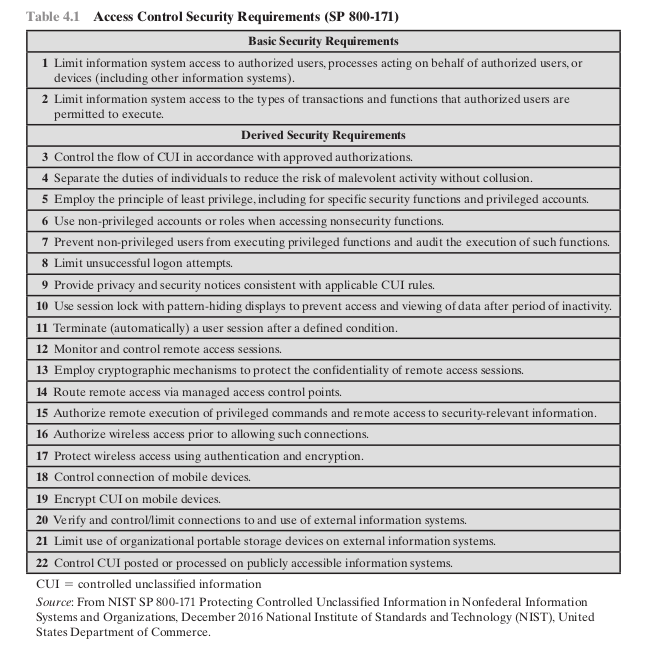
\includegraphics[width=14cm, keepaspectratio]{Bistarelli/img/cap_4/tabella4.1.png}
\end{figure}

In senso lato, tutta la sicurezza informatica riguarda il controllo degli accessi. Infatti, RFC 4949 definisce la sicurezza informatica come segue:

\begin{center}
    \textbf{Misure che implementano e assicurano servizi di sicurezza in un sistema informatico, in particolare quelle che assicurano il servizio di controllo degli accessi.}
\end{center}
\end{enumerate}
\newpage
\subsection{Contesto del controllo dell'accesso}
Oltre al controllo d'accesso, questo contesto coinvolge le seguenti entità e funzioni:
\begin{itemize}
    \item \textbf{Autenticazione}
    
    Verifica che le credenziali di un utente o di un'altra entità del sistema siano valide.
    
    \item \textbf{Autorizzazione}
    
    La concessione di un diritto o di un permesso ad un'entità di sistema per accedere una risorsa del sistema. Questa funzione determina chi è affidabile per un determinato scopo.
    
    \item \textbf{Audit}
    
    Una revisione ed esame indipendente delle registrazioni e delle attività del sistema al fine di verificare l'adeguatezza dei controlli del sistema, di assicurare la conformità con con la politica stabilita e le procedure operative, per rilevare le violazioni della sicurezza, e per raccomandare qualsiasi cambiamento indicato nel controllo, nella politica e nelle procedure.

\end{itemize}
Un meccanismo di controllo dell'accesso media tra un utente (o un processo che esegue per conto di un utente) e le risorse di sistema, come applicazioni, sistemi operativi, firewall, router, file e database. Il sistema deve prima autenticare un'entità che cerca l'accesso. Tipicamente, la funzione di autenticazione determina se l'utente è permesso di accedere al sistema. Poi la funzione di controllo dell'accesso determina se l'accesso specifico richiesto da questo utente è permesso. Un amministratore di sicurezza mantiene un database un database di autorizzazioni che specifica quale tipo di accesso a quali risorse è permesso a questo utente. La funzione di controllo degli accessi consulta questo database per se concedere l'accesso. Una funzione di auditing monitora e tiene un registro degli accessi degli utenti alle risorse del sistema.
\singlespacing
In pratica, un certo numero di componenti può cooperare per condividere la funzione di controllo la funzione di controllo degli accessi. Tutti i sistemi operativi hanno almeno un rudimentale, e in molti casi un componente di controllo degli accessi abbastanza robusto. I pacchetti di sicurezza aggiuntivi possono integrare le capacità di controllo d'accesso native del sistema operativo. Applicazioni particolari o utilità, come un sistema di gestione di database, incorporano anche funzioni di controllo degli accessi funzioni di controllo degli accessi. Dispositivi esterni, come i firewall, possono anche fornire servizi di controllo dell'accesso.
\newpage
\subsection{Politiche di controllo dell'accesso}
Una politica di controllo degli accessi, che può essere incorporata in un database di autorizzazioni, quali tipi di accesso sono permessi, in quali circostanze e da chi.
\singlespacing
Le politiche di controllo dell'accesso sono generalmente raggruppate nelle seguenti categorie:
\begin{itemize}
    \item \textbf{Controllo dell'accesso discrezionale (DAC)}
    
    Controlla l'accesso in base all'identità del richiedente e su regole di accesso (autorizzazioni) che stabiliscono cosa i richiedenti sono (o non sono)autorizzati a fare. Questa politica è definita discrezionale perché un'entità può avere diritti di accesso che permettono all'entità, di sua spontanea volontà, di un'altra entità di accedere a qualche risorsa.
    
    \item \textbf{Controllo di accesso obbligatorio (MAC)}
    
    
    Controlla l'accesso basandosi sul confronto delle etichette di sicurezza (che indicano quanto sono sensibili o critiche le risorse del sistema) con le autorizzazioni di sicurezza (che indicano le entità del sistema). con le autorizzazioni di sicurezza (che indicano che le entità del sistema sono autorizzate ad accedere a certe risorse). risorse). Questa politica è definita obbligatoria perché un'entità che ha l'autorizzazione di accedere a una risorsa non può, solo per sua volontà, permettere a un'altra entità di accedere a quella risorsa.
    
    \item \textbf{Controllo di accesso basato sui ruoli (RBAC)}
    
    Controlla l'accesso in base ai ruoli che gli utenti hanno all'interno del sistema e su regole che stabiliscono quali accessi sono permessi agli utenti in determinati ruoli.
    
    \item \textbf{Controllo di accesso basato sugli attributi (ABAC)}
    
    Controlla l'accesso in base agli attributi dell'utente, della risorsa a cui accedere e delle condizioni ambientali correnti.
\end{itemize}
\singlespacing
Queste quattro politiche non si escludono a vicenda. Un meccanismo di controllo degli accessi può impiegare due o anche tutte e tre queste politiche per coprire diverse classi di risorse di sistema.
\newpage
\subsection{Soggetti oggetti e diritti d'accesso}
Gli elementi di base del controllo d'accesso sono: soggetto, oggetto e diritto d'accesso.
\singlespacing
Un soggetto è un'entità capace di accedere agli oggetti. In generale, il concetto di soggetto equivale a quello di processo. Qualsiasi utente o applicazione ottiene effettivamente l'accesso a un oggetto per mezzo di un processo che rappresenta quell'utente o applicazione. Il processo assume gli attributi dell'utente, come i diritti di accesso.
\singlespacing
Un soggetto è tipicamente ritenuto responsabile delle azioni che ha iniziato, e un audit trail può essere usato per registrare l'associazione di un soggetto con azioni rilevanti per la sicurezza eseguite su un oggetto dal soggetto.
I sistemi di controllo dell'accesso di base definiscono tipicamente tre classi di soggetti, con diritti di accesso diversi per ogni classe:
\begin{itemize}
    \item \textbf{Propietario:} può essere il creatore di una risorsa, come un file. Per le risorse di sistema, la proprietà può appartenere ad un amministratore di sistema. Per le risorse del progetto, l'amministratore o il un amministratore di progetto o un leader può essere assegnato la proprietà.
    
    \item \textbf{Gruppo:} In aggiunta ai privilegi assegnati ad un proprietario, ad un gruppo nominato di utenti possono anche essere concessi diritti di accesso, in modo tale che l'appartenenza al gruppo sufficiente per esercitare questi diritti di accesso. Nella maggior parte degli schemi, un utente può appartenere a più gruppi.
    
    \item \textbf{Mondo:} Il minimo di accesso è concesso agli utenti che sono in grado di accedere al sistema ma non sono inclusi nelle categorie proprietario e gruppo per questa risorsa.
\end{itemize}
Un oggetto è una risorsa il cui accesso è controllato. In generale, un oggetto è un'entità usata per contenere e/o ricevere informazioni.
\singlespacing
Il numero e i tipi di oggetti da proteggere con un sistema di controllo degli accessi dipende dall'ambiente in cui opera il controllo degli accessi e dal compromesso tra sicurezza da un lato e complessità, carico di lavoro e facilità d'uso dall'altro.
\singlespacing
Un diritto di accesso descrive il modo in cui un soggetto può accedere a un oggetto.
\singlespacing
I diritti di accesso potrebbero includere quanto segue:
\begin{itemize}
    \item \textbf{Leggere:} L'utente può visualizzare le informazioni in una risorsa di sistema (ad esempio, un file, record selezionati record in un file, campi selezionati all'interno di un record, o qualche combinazione). Lettura l'accesso include la possibilità di copiare o stampare.
    
    \item \textbf{Scrittura:} L'utente può aggiungere, modificare o cancellare dati in una risorsa di sistema (ad esempio, file, record, programmi). L'accesso in scrittura include l'accesso in lettura.
    
    \item \textbf{Eseguire:} L'utente può eseguire programmi specifici.
    
    \item \textbf{Cancellare:} L'utente può cancellare certe risorse di sistema, come file o record.
    
    \item \textbf{Creare:} L'utente può creare nuovi file, record o campi.
    
    \item \textbf{Cercare:} L'utente può elencare i file in una directory o altrimenti cercare nella directory.
\end{itemize}
\subsection{Controllo dell'accesso discrezionale}
Come si è detto in precedenza, uno schema di controllo di accesso discrezionale è uno schema in cui un'entità può ricevere diritti di accesso che le permettono, per sua volontà, di permettere a un'altra entità di accedere a qualche risorsa. Un approccio generale al DAC, come esercitato da un sistema operativo o da un sistema di gestione di database, è quello di una matrice di accesso.
\begin{center}
    \textbf{Una dimensione della matrice consiste in soggetti identificati che possono tentare l'accesso alle risorse.}
\end{center}
Tipicamente, questa lista consisterà di singoli utenti o gruppi di utenti anche se l'accesso potrebbe essere controllato per terminali, apparecchiature di rete, host, o applicazioni invece di o in aggiunta agli utenti. L'altra dimensione elenca gli oggetti a cui si può accedere. Al massimo livello di dettaglio, gli oggetti possono essere singoli dati campi di dati. Raggruppamenti più aggregati, come record, file o anche l'intero database, possono anche essere oggetti nella matrice. Ogni voce nella matrice indica i diritti di accesso di un particolare soggetto per un particolare oggetto.

\begin{figure}[H]
	\centering
    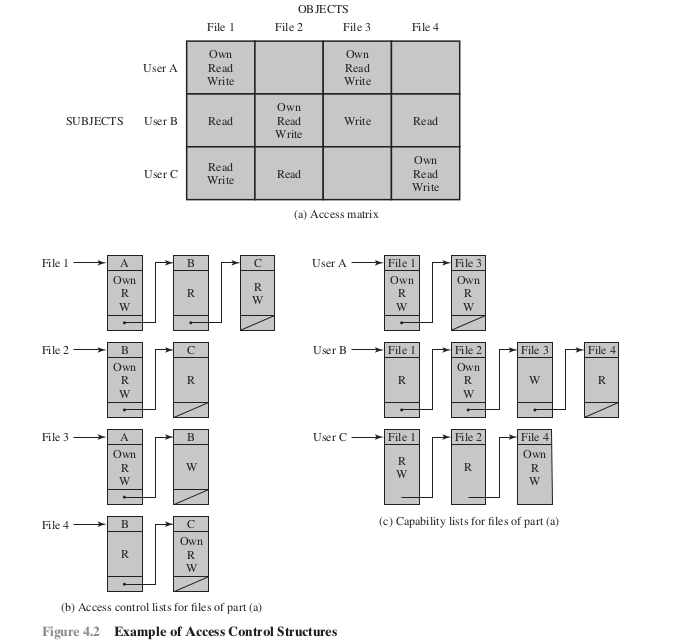
\includegraphics[width=14cm, keepaspectratio]{Bistarelli/img/cap_4/figura4.2.png}
\end{figure}

Così, l'utente A possiede i file 1 e 3 e ha diritti di accesso in lettura e scrittura a questi file. L'utente B ha diritti di accesso in lettura al file 1, e così via.

\singlespacing

In pratica, una matrice di accesso è di solito sparsa e viene implementata con la decomposizione in uno dei due modi. La matrice può essere decomposta per colonne, ottenendo liste di controllo degli accessi (ACL) (vedi Figura 4.2b). Per ogni oggetto, una ACL elenca gli utenti e i loro diritti di accesso consentiti. L'ACL può contenere una voce di default, o pubblica. Questo permette agli utenti che non sono esplicitamente elencati come aventi diritti speciali di avere un set di diritti. L'insieme predefinito di diritti dovrebbe sempre seguire la regola del minimo privilegio o accesso in sola lettura, a seconda del caso. Gli elementi della lista possono includere singoli utenti così come gruppi di utenti.

\singlespacing

Quando si vuole determinare quali soggetti hanno quali diritti di accesso ad una particolare risorsa, le ACL sono convenienti, perché ogni ACL fornisce le informazioni per una data risorsa. Tuttavia, questa struttura di dati non è conveniente per determinare i diritti di accesso disponibili per uno specifico utente.

\singlespacing

La decomposizione per righe produce i capability ticket (vedi Figura 4.2c).

\singlespacing

Un capability è un ticket di capacità specifica gli oggetti e le operazioni autorizzate per un particolare utente. Ogni utente ha un certo numero di ticket e può essere autorizzato a prestarli o darli ad altri. Poiché i ticket possono essere dispersi nel sistema, presentano un problema di sicurezza maggiore rispetto alle liste di controllo degli accessi. L'integrità del ticket deve essere protetta e garantita (di solito dal sistema operativo). In particolare, il ticket deve essere non falsificabile. Un modo per ottenere ciò è quello di avere il sistema operativo che tiene tutti i ticket per conto degli utenti. Questi biglietti dovrebbero essere tenuti in una regione di memoria inaccessibile agli utenti. Un'altra alternativa è includere un token non falsificabile nella capacità. Questo potrebbe essere una grande password casuale, o un codice crittografico di autenticazione del messaggio. Questo valore è verificato dalla risorsa ogni volta che viene richiesto l'accesso. Questa forma di capability ticket è appropriata per Questa forma di capability ticket è appropriata per l'uso in un ambiente distribuito, quando la sicurezza del suo contenuto non può essere garantita. Gli aspetti convenienti e scomodi dei capability ticket sono l'opposto di quelli delle ACL. È facile determinare l'insieme dei diritti di accesso che un dato utente ha, ma è più difficile determinare l'elenco degli utenti con diritti di accesso specifici per una risorsa specifica.

\singlespacing

Una tabella di autorizzazione contiene una riga per un diritto di accesso di un soggetto ad una risorsa. Ordinare o accedere alla tabella per soggetto è equivalente a una lista di capacità. Ordinare o l'accesso alla tabella per oggetto è equivalente ad una ACL. Un database relazionale può facilmente implementare una tabella di autorizzazione di questo tipo.

\begin{figure}[H]
	\centering
    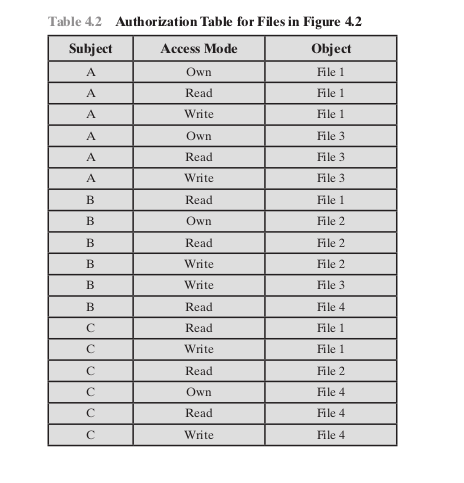
\includegraphics[width=14cm, keepaspectratio]{Bistarelli/img/cap_4/tabella4.2.png}
\end{figure}
\newpage
\subsection{Un modello di controllo d'accesso}
Questa sezione introduce un modello generale per DAC sviluppato da Lampson, Graham, e Denning. Il modello presuppone un insieme di soggetti, un insieme di oggetti e un insieme di regole che governano l'accesso dei soggetti agli oggetti. Definiamo lo stato di protezione di un sistema come l'insieme di informazioni, in un dato momento, che specifica i diritti di accesso per ogni soggetto rispetto a ogni oggetto.

\singlespacing

Noi Possiamo identificare tre requisiti: rappresentare lo stato di protezione, far rispettare i diritti di accesso e permettere ai soggetti di alterare lo stato di protezione in certi modi. Il modello affronta tutti e tre i requisiti, dando una descrizione generale e logica di un sistema DAC.

\singlespacing

Per rappresentare lo stato di protezione, estendiamo l'universo di oggetti nella matrice di controllo degli accessi per includere quanto segue:
\begin{itemize}
    \item \textbf{Processi:} I diritti di accesso includono la capacità di cancellare un processo, fermare (bloccare) e svegliare un processo.

    \item \textbf{Dispositivi:} I diritti di accesso includono la capacità di leggere/scrivere il dispositivo, di controllare il suo funzionamento (ad esempio, una ricerca su disco), e di bloccare/sbloccare il dispositivo per l'uso.
    
    \item \textbf{Luoghi o regioni di memoria:} I diritti di accesso includono la capacità di leggere/scrivere certe regioni di memoria che sono protette in modo tale che il default è di disabilitare l'accesso.
    
    \item \textbf{Soggetti:} I diritti di accesso rispetto ad un soggetto hanno a che fare con la capacità di concedere o cancellare i diritti di accesso di quel soggetto ad altri oggetti, come spiegato successivamente.
\end{itemize}
La figura 4.3 è un esempio. Per una matrice di controllo di accesso A, ogni voce A[S, X] contiene stringhe, chiamate attributi di accesso, che specificano i diritti di accesso del soggetto S all per l'oggetto X. Per esempio, nella figura 4.3, S1 può leggere il file F1, perché 'read' appare in A[S1, F1]. Da un punto di vista logico o funzionale, un modulo di controllo degli accessi separato è associato ad ogni tipo di oggetto (vedi figura 4.4). Il modulo valuta ogni Il modulo valuta ogni richiesta di un soggetto di accedere a un oggetto per determinare se il diritto di accesso esiste. Un tentativo di accesso innesca i seguenti passi:
\begin{enumerate}
    \item Un soggetto S0 emette una richiesta di tipo a per l'oggetto X.
    
    \item La richiesta fa sì che il sistema (il sistema operativo o un modulo di interfaccia di controllo degli accessi di qualche tipo) a generare un messaggio della forma (S0, a, X) al controllore per X.
    
    \item Il controllore interroga la matrice di accesso A per determinare se a è in A[S0, X].
\end{enumerate}

\begin{figure}[H]
	\centering
    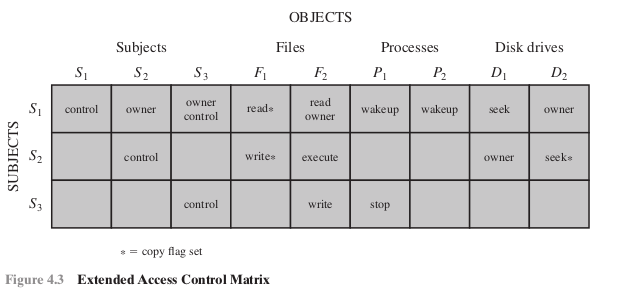
\includegraphics[width=14cm, keepaspectratio]{Bistarelli/img/cap_4/figura4.3.png}
\end{figure}

In caso affermativo, l'accesso è permesso; in caso contrario, l'accesso è negato e si verifica una violazione della protezione si verifica una violazione della protezione. La violazione dovrebbe innescare un avvertimento e un'azione appropriata.

\singlespacing

La figura 4.4 suggerisce che ogni accesso di un soggetto ad un oggetto è mediato dal controllore per quell'oggetto, e che la decisione del controllore è basata sul contenuto attuale della matrice. Inoltre, alcuni soggetti hanno l'autorità di apportare modifiche specifiche alla matrice di accesso. Una richiesta di modifica della matrice di accesso è trattata come un accesso alla matrice, con le singole voci della matrice trattate come oggetti.

\singlespacing

Tali accessi sono mediati da un controllore della matrice di accesso, che controlla gli aggiornamenti alla matrice. Il modello include anche un insieme di regole che governano le modifiche alla matrice di accesso come mostrato nella tabella 4.3. A questo scopo, introduciamo i diritti di accesso "proprietario e 'controllo' e il concetto di flag di copia, come spiegato nei paragrafi successivi.

\singlespacing

Le prime tre regole riguardano il trasferimento, la concessione e la cancellazione dei diritti di accesso. Supponiamo che la voce a* esista in A[S0, X]. Questo significa che S0 ha il diritto di accesso a al soggetto X e, a causa della presenza del flag di copia, può trasferire questo diritto, con o senza con o senza flag di copia, ad un altro soggetto. La regola R1 esprime questa capacità. Un soggetto potrebbe trasferire il diritto di accesso senza il flag di copia se ci fosse la preoccupazione che il nuovo soggetto potrebbe trasferire maliziosamente il diritto ad un altro soggetto che non dovrebbe avere quel diritto di accesso. Per esempio, S1 può mettere 'read' o 'read*' in qualsiasi voce della matrice in nella colonna F1. La regola R2 afferma che se S0 è designato come proprietario dell'oggetto X, allora S0 può concedere un diritto di accesso a quell'oggetto per qualsiasi altro soggetto. La regola R2 afferma che che se S0 è designato come proprietario dell'oggetto X, allora S0 può concedere un diritto di accesso a quell'oggetto per qualsiasi altro soggetto.

\singlespacing

\paragraph{La regola R2} afferma che S0 può aggiungere qualsiasi diritto di accesso ad A[S, X] per qualsiasi S, se S0 ha accesso "proprietario" a X. La regola R3 permette a S0 di cancellare qualsiasi diritto di accesso da qualsiasi voce della matrice in una riga per la quale S0 controlla il soggetto, e per qualsiasi voce della matrice in una colonna per la quale S0 possiede l'oggetto.

\singlespacing

\paragraph{La regola R4} permette ad un soggetto di leggere quella porzione di matrice che possiede o controlla.

\singlespacing

Le restanti regole della tabella 4.3 regolano la creazione e la cancellazione di soggetti e oggetti.

\singlespacing

\paragraph{La regola R5} afferma che ogni soggetto può creare un nuovo oggetto, che possiede, e può quindi concedere e cancellare l'accesso all'oggetto. Secondo la regola R6, il proprietario di un oggetto può distruggere l'oggetto, con la conseguente cancellazione della colonna corrispondente della matrice di accesso.

\singlespacing

\paragraph{La regola R7} permette a qualsiasi soggetto di creare un nuovo soggetto; il creatore è proprietario del nuovo soggetto e il nuovo soggetto ha accesso di controllo su se stesso.

\singlespacing

\paragraph{La regola R8} permette al proprietario di un soggetto di cancellare la riga e la colonna (se ci sono colonne di soggetti) della matrice di accesso designata da quel soggetto.

\singlespacing

L'insieme di regole nella Tabella 4.3 è un esempio dell'insieme di regole che potrebbero essere definite per un sistema di controllo degli accessi. I seguenti sono esempi di regole aggiuntive o alternative

\begin{figure}[H]
	\centering
    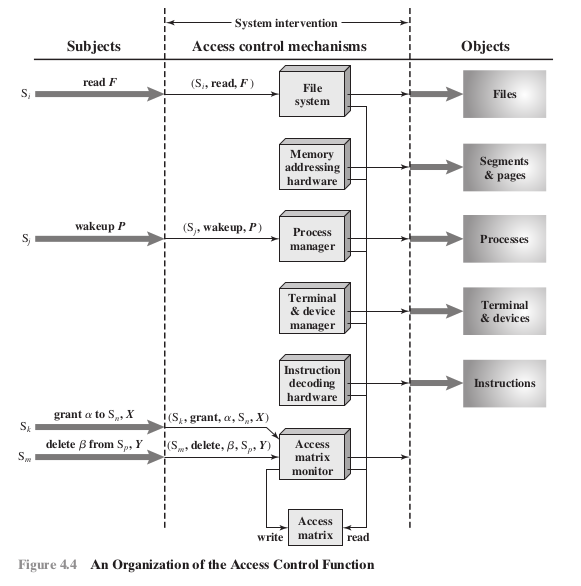
\includegraphics[width=14cm, keepaspectratio]{Bistarelli/img/cap_4/figura4.4.png}
\end{figure}

\begin{figure}[H]
	\centering
    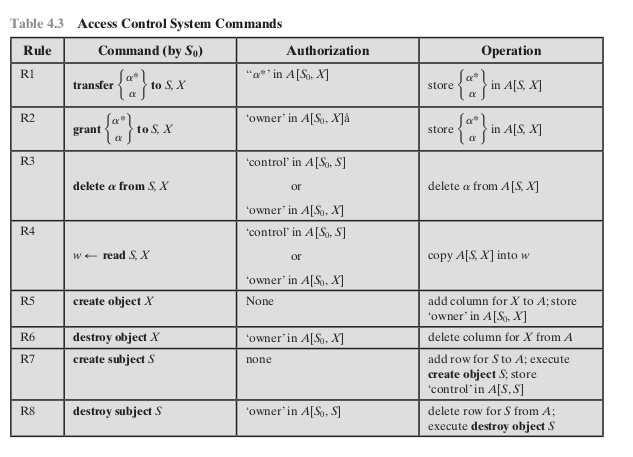
\includegraphics[width=14cm, keepaspectratio]{Bistarelli/img/cap_4/tabella4.3.png}
\end{figure}
\section{Esempio: Controllo di accesso ai file Unix}
Tutti i tipi di file UNIX sono amministrati dal sistema operativo per mezzo di inode.
\singlespacing
\textbf{Un inode} (nodo indice) è una struttura di controllo che contiene le informazioni chiave necessarie al sistema operativo per un particolare file. Diversi nomi di file possono essere associati ad un singolo inode, ma un inode attivo è associato esattamente ad un file, e ogni file è controllato esattamente da un inode. Gli attributi del file così come i suoi permessi e altre informazioni di controllo sono memorizzati nell'inode. Sul disco, c'è una tabella di inode, o lista di inode, che contiene gli inode di tutti i file nel file sistema. Quando un file viene aperto, il suo inode viene portato nella memoria principale e memorizzato in una tabella di inode residente in memoria.
\singlespacing
Le directory sono strutturate in un albero gerarchico. Ogni directory può contenere file e/o altre directory. Una directory che si trova all'interno di un'altra directory viene una sottodirectory. Una directory è semplicemente un file che contiene una lista di nomi di file più puntatori agli inode associati. Così, associato ad ogni directory c'è il proprio inode.
\subsection{Controllo di accesso ai file UNIX tradizionale}
La maggior parte dei sistemi UNIX dipende, o almeno si basa, sullo schema di controllo dell'accesso ai file introdotto con le prime versioni di UNIX. Ad ogni utente UNIX viene assegnato un unico numero di identificazione utente (ID utente). Un utente è anche membro di un gruppo primario, e possibilmente di un certo numero di altri gruppi, ciascuno identificato da un ID di gruppo. Quando un file viene creato, è designato come di proprietà di un particolare utente e contrassegnato dall'ID di quell'utente \textbf{ID DI QUELL'UTENTE}.
\singlespacing
Appartiene anche a un gruppo specifico, che inizialmente è o il gruppo primario del suo creatore, o il gruppo della sua directory madre se questa ha il permesso SetGID impostato. Associato ad ogni file c'è un insieme di 12 bit di protezione. L'ID del proprietario, l'ID del gruppo e i bit di protezione fanno parte dell'inode del file.
\singlespacing
Nove dei bit di protezione specificano i permessi di lettura, scrittura ed esecuzione per il proprietario del file, gli altri membri del gruppo a cui questo file appartiene e tutti gli altri utenti. Questi formano una gerarchia di proprietario, gruppo e tutti gli altri, con l'insieme di permessi più alto che viene usato. La figura 4.5a mostra un esempio in cui il proprietario del file ha accesso in lettura e scrittura; tutti gli altri membri del gruppo del file hanno accesso in lettura; e gli utenti esterni al gruppo non hanno diritti di accesso al file. Quando sono applicati ad una directory, i bit di lettura e scrittura garantiscono il diritto di elencare e creare/rinominare/cancellare file nella directory. Il bit di esecuzione garantisce il diritto di scendere nella directory o di cercare un nome di file.

\begin{figure}[H]
	\centering
    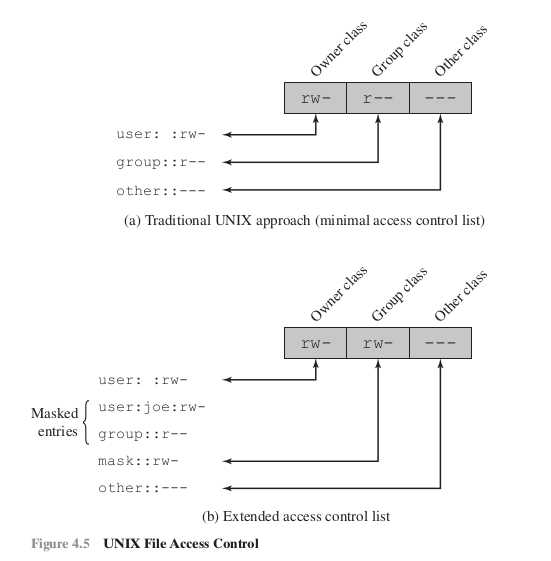
\includegraphics[width=14cm, keepaspectratio]{Bistarelli/img/cap_4/figura4-5.png}
\end{figure}

I tre bit rimanenti definiscono uno speciale comportamento aggiuntivo per i file o le directory. Due di questi sono i permessi "set user ID" (SetUID) e "set group ID" (SetGID) permessi. Se questi sono impostati su un file eseguibile, il sistema operativo funziona come segue.

\singlespacing

Quando un utente (con privilegi di esecuzione per questo file) esegue il file, il sistema alloca temporaneamente i diritti dell'ID dell'utente del creatore del file, o del gruppo del file, rispettivamente, a quelli dell'utente che esegue il file. Questi sono conosciuti come "ID utente effettivo" e "ID gruppo effettivo" e sono usati in aggiunta all'"ID utente reale" e all'"ID gruppo reale". "ID" e "ID gruppo reale" dell'utente in esecuzione quando si prendono decisioni di controllo dell'accesso per questo programma. Questa modifica è efficace solo mentre il programma è in esecuzione.

\singlespacing

Questa caratteristica permette la creazione e l'uso di programmi privilegiati che possono utilizzare file normalmente inaccessibili agli altri utenti. Permette agli utenti di accedere a certi file in modo con controllato. In alternativa, quando applicato ad una directory, il permesso SetGID indica che i file appena creati erediteranno il gruppo di questa directory. Il permesso SetUID viene ignorata.

\singlespacing

L'ultimo bit di permesso è il bit "appiccicoso". Quando è impostato su un file, originariamente indica che il sistema dovrebbe mantenere il contenuto del file in memoria dopo l'esecuzione. Questo non è più usato. Quando è applicato ad una directory, però, specifica che solo il proprietario di qualsiasi file nella directory può rinominare, spostare o cancellare quel file. Questo è utile per gestire i file nelle directory temporanee condivise.

\singlespacing

Un particolare ID utente è designato come "superutente". Il superutente è esente dai soliti vincoli di controllo dell'accesso ai file e ha accesso a tutto il sistema. Qualsiasi programma che è posseduto da, e SetUID a, il "superutente" garantisce potenzialmente un accesso illimitato al sistema accesso al sistema a qualsiasi utente che esegua quel programma. Quindi è necessaria una grande attenzione quando si scrivono tali programmi.

\singlespacing

Questo schema di accesso è adeguato quando i requisiti di accesso ai file si allineano con gli utenti e un numero modesto di gruppi di utenti. Per esempio, supponiamo che un utente voglia dare l'accesso in lettura per il file X agli utenti A e B, e l'accesso in lettura per il file Y agli utenti B e C.

\singlespacing

Avremmo bisogno di almeno due gruppi di utenti, e l'utente B dovrebbe appartenere ad entrambi gruppi per poter accedere ai due file. Tuttavia, se c'è un gran numero di diversi raggruppamenti di utenti che richiedono una serie di diritti di accesso a diversi file, allora potrebbe essere necessario un numero molto grande di gruppi può essere necessario per fornire questo. Questo diventa rapidamente ingombrante e difficile da gestire, se possibile.

\singlespacing

Un modo per superare questo problema è usare le liste di controllo degli accessi, che sono fornite nella maggior parte dei moderni sistemi UNIX. Un ultimo punto da notare è che il tradizionale schema di controllo di accesso ai file UNIX implementa una semplice struttura di dominio di protezione. Un dominio è associato con l'utente, e cambiare il dominio corrisponde a cambiare temporaneamente l'ID dell'utente.
\newpage
\subsection{Liste di controllo d'accesso in UNIX}
Molti moderni sistemi operativi UNIX e basati su UNIX supportano le liste di controllo degli accessi, inclusi FreeBSD, OpenBSD, Linux e Solaris. In questa sezione, descriviamo FreeBSD, ma altre implementazioni hanno essenzialmente le stesse caratteristiche e la stessa interfaccia. La caratteristica è indicata come lista di controllo di accesso estesa, mentre il tradizionale approccio UNIX UNIX tradizionale è indicato come lista di controllo dell'accesso minima.

\singlespacing

\textbf{FreeBSD} permette all'amministratore di assegnare una lista di ID utente UNIX e ad un file usando il comando setfacl. Qualsiasi numero di utenti e gruppi può essere associato ad un file, ognuno con tre bit di protezione (lettura, scrittura, esecuzione), offrendo un meccanismo flessibile per l'assegnazione dei diritti di accesso. Un file non ha bisogno di avere un ACL ma può essere protetto solo dal tradizionale meccanismo di accesso ai file UNIX. I file FreeBSD includono un ulteriore bit di protezione che indica se il file ha una ACL estesa.

FreeBSD e la maggior parte delle implementazioni UNIX che supportano le ACL estese usano la seguente strategia (ad esempio, Figura 4.5b):
\begin{enumerate}
    \item La classe del proprietario e le altre voci di classe nel campo dei permessi a 9 bit hanno lo stesso stesso significato che nel caso dell'ACL minima.
    
    \item La voce group class specifica i permessi per il gruppo proprietario di questo file.


Questi permessi rappresentano i permessi massimi che possono essere assegnati a utenti nominati o gruppi nominati, diversi dall'utente proprietario. In quest'ultimo ruolo, la voce classe di gruppo funziona come una maschera.

    \item Altri utenti e gruppi nominati possono essere associati al file
    
Ognuno con un campo di autorizzazione a 3 bit. I permessi elencati per un utente o un gruppo gruppo sono confrontati con il campo della maschera. Qualsiasi permesso per l'utente o il gruppo gruppo che non è presente nel campo della maschera non è permesso.
\end{enumerate}
Quando un processo richiede l'accesso ad un oggetto del file system, vengono eseguiti due passi.

\begin{enumerate}
    \item \textbf{Passo seleziona la voce ACL che più si avvicina al processo richiedente.}
    
Il sito ACL vengono esaminate nel seguente ordine: proprietario, utenti nominati, gruppi (proprietari o con nome) gruppi, altri. Solo una singola voce determina l'accesso.

    \item \textbf{Passo controlla se la voce voce corrispondente contiene sufficienti permessi.}

Un processo può essere membro di più di un gruppo; quindi più di una voce di gruppo può corrispondere. Se una di queste voci di gruppo corrispondenti gruppo corrispondente contiene i permessi richiesti, ne viene scelto uno che contiene i permessi richiesti (il risultato è lo stesso indipendentemente dalla voce scelta). Se nessuna delle delle voci di gruppo corrispondenti contiene i permessi richiesti, l'accesso sarà negato indipendentemente dalla voce scelta.
\end{enumerate}
\newpage
\section{Controllo d'accesso basato sul ruolo}

\begin{figure}[H]
	\centering
    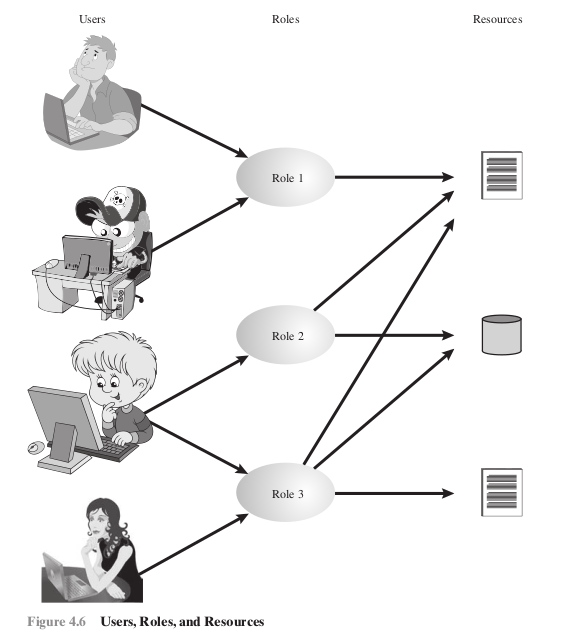
\includegraphics[width=14cm, keepaspectratio]{Bistarelli/img/cap_4/figura4.6.png}
\end{figure}

\begin{figure}[H]
	\centering
    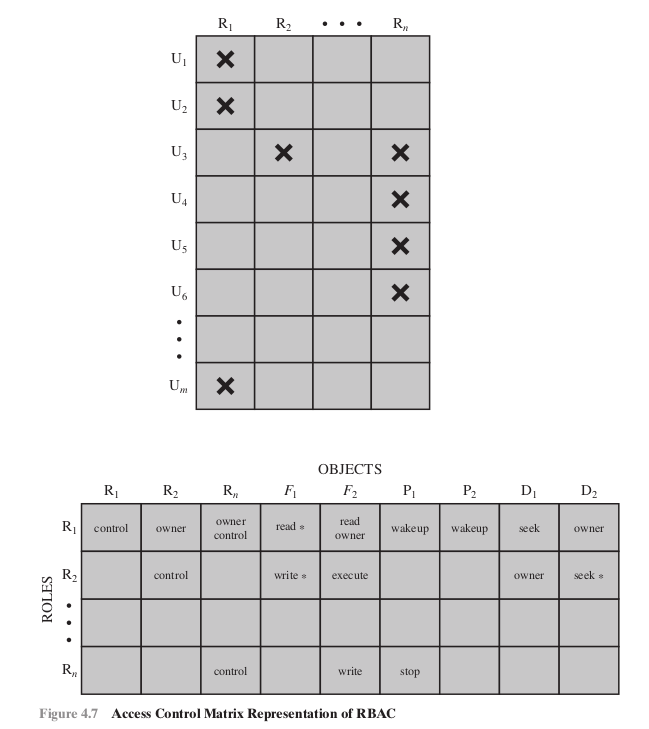
\includegraphics[width=14cm, keepaspectratio]{Bistarelli/img/cap_4/figura4.7.png}
\end{figure}


I sistemi DAC tradizionali definiscono i diritti di accesso dei singoli utenti e dei gruppi di utenti. Al contrario, RBAC si basa sui ruoli che gli utenti assumono in un sistema piuttosto che sull'identità dell'utente. Tipicamente, i modelli RBAC definiscono un ruolo come una funzione lavorativa all'interno un'organizzazione. I sistemi RBAC assegnano i diritti di accesso ai ruoli invece che ai singoli utenti. A loro volta, gli utenti sono assegnati a diversi ruoli, sia staticamente che dinamicamente, secondo le loro responsabilità.

\singlespacing

RBAC ora gode di un ampio uso commerciale e rimane un'area di ricerca attiva. Il National Institute of Standards and Technology (NIST) ha emesso uno standard, FIPS PUB 140-3 (Security Requirements for Cryptographic Modules, settembre 2009), che richiede il supporto per il controllo degli accessi e l'amministrazione attraverso i ruoli. La relazione degli utenti con i ruoli è molti a molti, così come la relazione dei ruoli alle risorse o agli oggetti del sistema (vedi Figura 4.6). L'insieme degli utenti cambia, in alcuni ambienti frequentemente, e l'assegnazione di un utente a uno o più ruoli può anche essere dinamico. L'insieme dei ruoli nel sistema nella maggior parte degli ambienti è relativamente statico, con solo occasionali aggiunte o cancellazioni. Ogni ruolo avrà diritti di accesso specifici a una o più risorse. L'insieme delle risorse e i diritti di accesso specifici associati con un particolare ruolo è probabile che cambino raramente.

\singlespacing

Possiamo usare la rappresentazione della matrice di accesso per rappresentare gli elementi chiave di un sistema RBAC in termini semplici, come mostrato nella figura 4.7. La matrice superiore mette in relazione i singoli utenti ai ruoli. Tipicamente ci sono molti più utenti che ruoli. Ogni matrice voce della matrice è vuota o marcata, quest'ultima indica che l'utente è assegnato a questo ruolo. Si noti che un singolo utente può essere assegnato a più ruoli (più di un segno in una riga) e più utenti possono essere assegnati a un singolo ruolo (più di un segno in una colonna). La matrice inferiore ha la stessa struttura della matrice di controllo degli accessi DAC, con i ruoli come soggetti. Tipicamente, ci sono pochi ruoli e molti oggetti, o risorse. In questa matrice, le voci sono i diritti di accesso specifici dei ruoli. Si noti che un ruolo può essere trattato come un oggetto, permettendo la definizione di gerarchie di ruoli.

\singlespacing

\textbf{RBAC} si presta ad un'efficace implementazione del principio del minimo privilegio, a cui si fa riferimento nel capitolo 1. Ogni ruolo dovrebbe contenere l'insieme minimo di diritti di accesso necessari per quel ruolo. Un utente viene assegnato ad un ruolo che gli permette di eseguire solo ciò che è richiesto per quel ruolo. Più utenti assegnati allo stesso ruolo godono dello stesso insieme minimo di diritti di accesso.
\newpage
\subsection{Modelli di riferimento RBAC}

\begin{figure}[H]
	\centering
    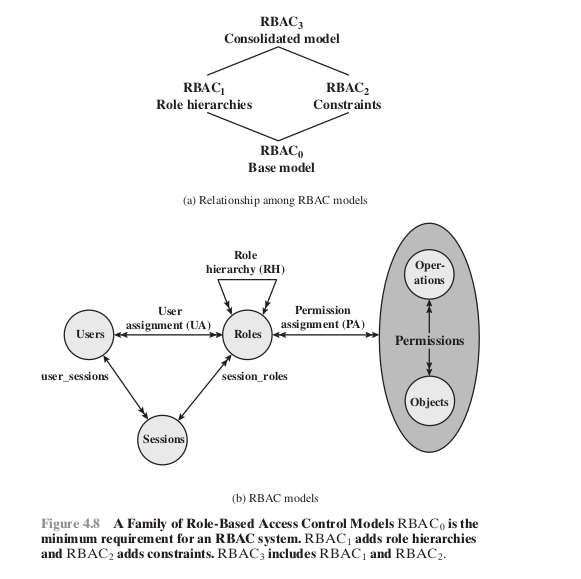
\includegraphics[width=14cm, keepaspectratio]{Bistarelli/img/cap_4/figura4.8.png}
\end{figure}

\begin{figure}[H]
	\centering
    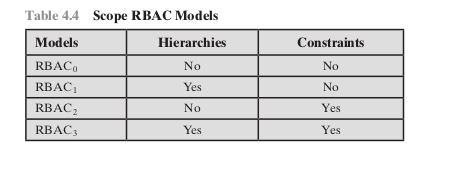
\includegraphics[width=14cm, keepaspectratio]{Bistarelli/img/cap_4/tabella4.4.png}
\end{figure}

Una varietà di funzioni e servizi possono essere inclusi sotto l'approccio generale RBAC approccio. Per chiarire i vari aspetti di RBAC, è utile definire un insieme di modelli astratti modelli astratti di funzionalità RBAC.

\singlespacing

Definisce una famiglia di modelli di riferimento che è servita come base per gli sforzi di standardizzazione in corso. Questa famiglia consiste di quattro modelli che sono correlati tra loro, come mostrato nella Figura 4.8a e nella Tabella 4.4. RBAC 0 contiene la funzionalità minima per un sistema RBAC.

\singlespacing

RBAC 1 include le funzionalità di RBAC 0 e aggiunge le gerarchie dei ruoli, che permettono a un ruolo di ereditare i permessi da un altro ruolo. RBAC 2 include RBAC 0 e aggiunge vincoli, che limitano i modi in cui i componenti di un sistema RBAC possono essere configurati. RBAC 3 contiene la funzionalità di RBAC 0, RBAC1 e RBAC2.

\singlespacing

\paragraph{Modello base-RBAC0}

Figura 4.8b, senza la gerarchia dei ruoli e i vincoli, contiene i quattro tipi di entità in un sistema RBAC 0:
\begin{itemize}

    \item \textbf{Utente:} un individuo che ha accesso a questo sistema informatico. Ogni individuo ha un ID utente associato.
    
    \item \textbf{Ruolo:} Una funzione di lavoro nominata all'interno dell'organizzazione che controlla questo sistema informatico. Tipicamente, associato ad ogni ruolo c'è una descrizione dell'autorità e della responsabilità conferite a questo ruolo, e a qualsiasi utente che assume questo ruolo.
    
    \item \textbf{Permesso:} Un'approvazione di una particolare modalità di accesso a uno o più oggetti. Termini equivalenti sono diritto di accesso, privilegio e autorizzazione.
    
    \item \textbf{Sessione:} Una mappatura tra un utente e un sottoinsieme attivato dell'insieme di ruoli a cui l'utente è assegnato.
    
\end{itemize}

Le linee con le frecce nella figura 4.8b indicano relazioni, o mappature, con una freccia singola che ne indica una e una doppia che ne indica molte. Quindi, c'è una relazione molti-a-molti tra utenti e ruoli: Un utente può avere più ruoli, e più utenti possono essere assegnati a un singolo ruolo. Allo stesso modo, c'è una relazione molti a molti tra ruoli e permessi. Una sessione è usata per definire una relazione temporanea uno-a-molti tra un utente e uno o più ruoli a cui l'utente è stato assegnato. L'utente stabilisce una sessione con solo i ruoli necessari per un particolare compito; questo è un esempio del concetto di minimo privilegio. Le relazioni molti-a-molti tra utenti e ruoli e tra ruoli e permessi forniscono una flessibilità e granularità di assegnazione che non si trova negli schemi DAC convenzionali. Senza questa flessibilità e granularità, c'è un rischio maggiore che ad un utente possa essere concesso più accesso alle risorse di quanto sia necessario a causa del controllo limitato sui tipi di accesso che possono essere permessi. 
\newpage
\begin{center}
    \textbf{Gerarchie di ruolo-RBAC1}
\end{center}

Le gerarchie di ruolo forniscono un mezzo per riflettere la struttura gerarchica dei ruoli in un'organizzazione. Tipicamente, le funzioni lavorative con maggiore responsabilità hanno maggiore autorità per accedere alle risorse. Una funzione lavorativa subordinata può avere un sottoinsieme dei diritti di accesso della funzione lavorativa superiore. Le gerarchie di ruolo fanno uso del concetto di ereditarietà per permettere ad un ruolo di includere implicitamente i diritti di accesso associati ad un ruolo subordinato. La figura 4.9 è un esempio di diagramma di una gerarchia di ruoli. Per convenzione, i ruoli subordinati sono più in basso nel diagramma. Una linea tra due ruoli implica che il ruolo superiore include tutti i diritti di accesso del ruolo inferiore, così come altri diritti di accesso non disponibili al ruolo inferiore. Un ruolo può ereditare diritti di accesso da più ruoli subordinati. Per esempio, nella figura 4.9, il ruolo Project Lead include tutti i diritti di accesso del ruolo Production Engineer e del ruolo Quality Engineer. Più di un ruolo può ereditare dallo stesso ruolo subordinato. Per esempio, sia il ruolo Production Engineer che il ruolo Quality Engineer includono tutti i diritti di accesso del ruolo Engineer. Ulteriori diritti di accesso sono anche assegnati al ruolo Production Engineer, e un diverso insieme di diritti di accesso aggiuntivi sono assegnati al ruolo Quality ingegnere di qualità. Quindi, questi due ruoli hanno diritti di accesso che si sovrappongono, vale a dire i diritti di accesso diritti di accesso che condividono con il ruolo Engineer.

\begin{center}
    \textbf{Vincoli-RBAC2}
\end{center}

I vincoli forniscono un mezzo per adattare RBAC alle specifiche delle politiche amministrative e di sicurezza in un'organizzazione. Un vincolo è una relazione definita tra i ruoli o una condizione relativa ai ruoli. Esistono i seguenti tipi di vincoli: ruoli mutuamente esclusivi, cardinalità e ruoli prerequisiti. I ruoli mutuamente esclusivi sono ruoli tali che un utente può essere assegnato ad un solo ruolo nell'insieme. Questa limitazione potrebbe essere statica, o potrebbe essere dinamica, nel senso che ad un utente potrebbe essere assegnato solo uno dei ruoli nell'insieme per una sessione. Il vincolo reciprocamente esclusivo supporta una separazione di doveri e capacità all'interno un'organizzazione. Questa separazione può essere rafforzata o migliorata dall'uso di assegnazioni di permessi reciprocamente esclusivi. Con questo vincolo aggiuntivo, un insieme di ruoli mutuamente esclusivi ha le seguenti proprietà:

\begin{center}
    Un utente può essere assegnato ad un solo ruolo nell'insieme (sia durante una sessione staticamente).
Qualsiasi permesso (diritto di accesso) può essere concesso ad un solo ruolo dell'insieme.
\end{center}

\begin{figure}[H]
	\centering
    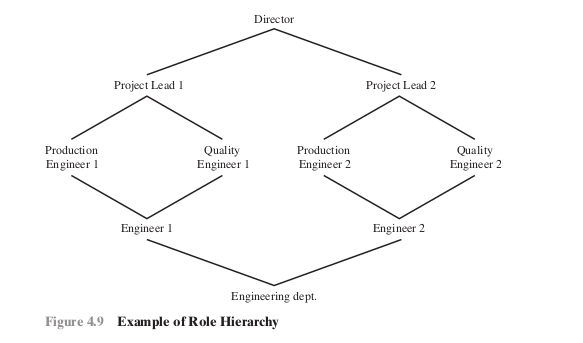
\includegraphics[width=14cm, keepaspectratio]{Bistarelli/img/cap_4/figura4.9.png}
\end{figure}


\singlespacing

Così, l'insieme dei ruoli reciprocamente esclusivi hanno permessi non sovrapposti. Se due utenti sono assegnati a ruoli diversi nell'insieme, allora gli utenti hanno permessi non sovrapposti permessi mentre assumono quei ruoli. Lo scopo dei ruoli mutuamente esclusivi è quello di aumentare la difficoltà di collusione tra individui con competenze diverse o funzioni funzioni lavorative divergenti per contrastare le politiche di sicurezza. La cardinalità si riferisce all'impostazione di un numero massimo rispetto ai ruoli. Uno di questi vincolo è quello di impostare un numero massimo di utenti che possono essere assegnati ad un dato ruolo.

Per esempio, un ruolo di capo progetto o un ruolo di capo reparto potrebbe essere limitato ad un singolo utente. Il sistema potrebbe anche imporre un vincolo sul numero di ruoli che un utente è assegnato, o il numero di ruoli che un utente può attivare per una singola sessione. Un'altra forma di vincolo è quella di impostare un numero massimo di ruoli che possono essere concessi un particolare permesso; questa potrebbe essere una tecnica desiderabile di mitigazione del rischio per un permesso sensitiva o potente.

\singlespacing

Un sistema potrebbe essere in grado di specificare un ruolo prerequisito, che impone che un utente possa essere assegnato a un particolare ruolo solo se è già assegnato a qualche altro ruolo specificato.

\singlespacing

Un prerequisito può essere usato per strutturare l'implementazione del concetto di minimo privilegio. In una gerarchia, potrebbe essere richiesto che un utente possa essere assegnato ad un ruolo (superiore) solo se gli è già stato assegnato un ruolo immediatamente inferiore. Per esempio, nella figura 4.9 un utente assegnato a un ruolo di Project Lead deve essere assegnato anche a ai ruoli subordinati Production Engineer e Quality Engineer. Quindi, se l'utente non ha bisogno di tutti i permessi del ruolo Project Lead per un dato compito, l'utente può invocare una sessione usando solo il ruolo subordinato richiesto. Si noti l'uso di prerequisiti legati al concetto di gerarchia richiede il modello RBAC 3.
\section{Controllo degli accessi basato su attributi}
Uno sviluppo relativamente recente nella tecnologia di controllo dell'accesso è il modello di controllo dell'accesso basato sugli attributi (ABAC). Un modello ABAC può definire autorizzazioni che esprimono condizioni su proprietà sia della risorsa che del soggetto. Per esempio, consideriamo una configurazione in cui ogni risorsa ha un attributo che identifica il soggetto che ha creato la risorsa. Quindi, una singola regola di accesso può specificare il privilegio del proprietario per tutti i creatori di ogni risorsa. La forza dell'approccio ABAC è la sua flessibilità e potenza espressiva. Sottolinea che il principale ostacolo alla sua adozione in sistemi reali è stata la preoccupazione per l'impatto della valutazione dei predicati su entrambe le proprietà della risorsa e dell'utente per ogni accesso.
\singlespacing
Tuttavia, per applicazioni come i servizi Web cooperanti e il cloud computing questo aumento del costo delle prestazioni è meno evidente perché c'è già un costo di prestazione relativamente alto per ogni accesso. Così, i servizi Web sono stati tecnologie innovative per l'implementazione di modelli ABAC, specialmente attraverso l'introduzione dell'eXtensible Access Control Markup Language (XAMCL) e c'è un notevole interesse nell'applicare il modello ABAC ai servizi cloud.
\singlespacing
Ci sono tre elementi chiave in un modello ABAC: gli attributi, che sono definiti per le entità in una configurazione; un modello di policy, che definisce le politiche ABAC; e il modello di architettura, che si applica alle politiche che impongono il controllo degli accessi.
\newpage
\subsection{Attributi}
Gli attributi sono caratteristiche che definiscono aspetti specifici del soggetto, dell'oggetto, delle condizioni ambientali e/o delle operazioni richieste che sono predefinite e preassegnate da un'autorità. Gli attributi contengono informazioni che indicano la classe di informa un nome e un valore (ad esempio, Class = HospitalRecordsAccess, Name = PatientInformationAccess, Value = MFBusinessHoursOnly).
\singlespacing
I seguenti sono i tre tipi di attributi nel modello ABAC:
\begin{itemize}
    \item \textbf{Attributi soggetto}
    
Un soggetto è un'entità attiva (ad esempio, un utente, un'applicazione, un processo o un dispositivo) che causa il flusso di informazioni tra gli oggetti o cambia lo stato del sistema. Ogni soggetto ha degli attributi associati che definiscono l'identità e le caratteristiche del soggetto. Tali attributi possono includere l'identificatore del soggetto identificatore, nome, organizzazione, titolo di lavoro e così via. Anche il ruolo di un soggetto può essere visto come un attributo.

    \item \textbf{Attributi dell'oggetto}
    
Un oggetto, chiamato anche risorsa, è un oggetto passivo (nel contesto della richiesta data) un'entità legata al sistema informativo (ad esempio, dispositivi, file, record, tabelle, processi, programmi, reti, domini) che contengono o ricevere informazioni. Come per i soggetti, gli oggetti hanno attributi che possono essere per prendere decisioni di controllo dell'accesso.

    \item \textbf{Attributi ambientali}
    
Questi attributi sono stati finora largamente ignorati nella maggior parte delle politiche di controllo degli accessi. Essi descrivono l'ambiente operativo, tecnico e anche ambiente o contesto situazionale in cui avviene l'accesso alle informazioni. Per esempio, attributi come la data e l'ora correnti, le attività correnti di virus/hacker e il livello di sicurezza della rete (ad esempio, Internet o intranet), non sono associati ad un particolare soggetto o ad una risorsa, ma possono comunque essere rilevanti nell'applicazione di una politica di controllo degli accessi. ABAC è un modello di controllo dell'accesso logico che si distingue perché controlla l'accesso agli oggetti valutando le regole contro gli attributi delle entità (soggetto e oggetto), le operazioni e oggetto), delle operazioni e dell'ambiente rilevanti per una richiesta. ABAC si basa sulla valutazione degli attributi del soggetto, degli attributi dell'oggetto e di una relazione forzata o una regola di controllo dell'accesso che definisce le operazioni consentite per le combinazioni di attributi di soggetto e oggetto in un dato ambiente.
\end{itemize}

\singlespacing

Tutte le soluzioni ABAC contengono queste capacità di base per valutare gli attributi e applicare regole o relazioni tra questi attributi. I sistemi ABAC sono in grado di applicare i concetti DAC, RBAC e concetti MAC. ABAC consente un controllo dell'accesso a grana fine, che permette un numero numero di input discreti in una decisione di controllo dell'accesso, fornendo un più grande insieme di possibili combinazioni di quelle variabili per riflettere un insieme più ampio e definitivo di possibili regole, politiche o restrizioni di accesso. Così, ABAC permette un numero illimitato numero illimitato di attributi da combinare per soddisfare qualsiasi regola di controllo dell'accesso. Inoltre, i sistemi ABAC possono essere implementati per soddisfare una vasta gamma di requisiti da dalle liste di controllo degli accessi di base a modelli di policy avanzati ed espressivi che sfruttano appieno la flessibilità dell'ABAC.
\newpage
\subsection{Architettura locìgica ABAC}
\begin{figure}[H]
	\centering
    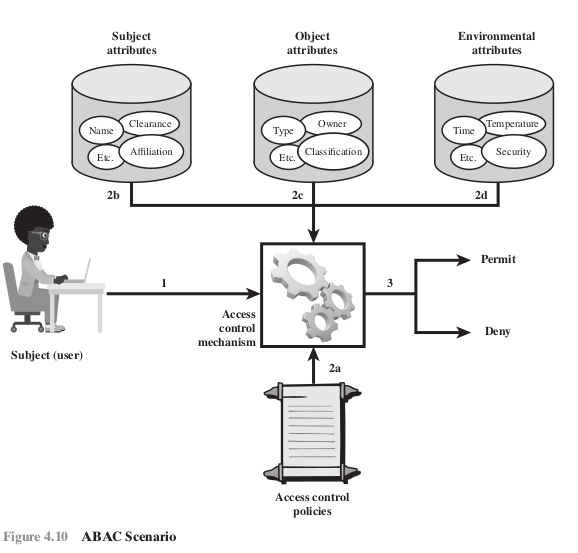
\includegraphics[width=14cm, keepaspectratio]{Bistarelli/img/cap_4/figura4.10.png}
\end{figure}

La figura 4.10 illustra in un'architettura logica i componenti essenziali di un sistema ABAC.

\singlespacing

Un accesso di un soggetto a un oggetto procede secondo i seguenti passi:

\begin{enumerate}

    \item Un soggetto richiede l'accesso ad un oggetto. Questa richiesta viene inoltrata ad un meccanismo di controllo meccanismo di controllo dell'accesso.
    
    \item Il meccanismo di controllo degli accessi è governato da un insieme di regole (2a) che sono definite da una politica di controllo dell'accesso preconfigurata. Sulla base di queste regole, il meccanismo di controllo dell'accesso valuta gli attributi del soggetto (2b), dell'oggetto (2c) e le condizioni ambientali (2d) per determinare l'autorizzazione.
    
    \item Il meccanismo di controllo dell'accesso concede al soggetto l'accesso all'oggetto se l'accesso è autorizzato, e nega l'accesso se non è autorizzato. È chiaro dall'architettura logica che ci sono quattro fonti indipendenti di informazioni utilizzate per la decisione di controllo dell'accesso.

\end{enumerate}

Il progettista del sistema può decidere quali attributi sono importanti per il controllo dell'accesso rispetto a soggetti, oggetti e condizioni ambientali. Il progettista del sistema o altra autorità può quindi definire politiche di controllo dell'accesso, sotto forma di regole, per qualsiasi combinazione desiderata di attri di soggetti, oggetti e condizioni ambientali.

\singlespacing

Dovrebbe essere evidente che questo approccio è molto potente e flessibile. Tuttavia, il costo, sia in termini di complessità della progettazione e dell'implementazione, e in termini di impatto sulle prestazioni, è probabile che superi quello di altri approcci di controllo dell'accesso. Questo è un compromesso che autorità di sistema deve fare.

\singlespacing

Rispetto a un modello DAC che usa liste di controllo degli accessi (ACL). Questa figura non solo illustra la complessità relativa dei due modelli, ma chiarisce anche i requisiti di fiducia dei due modelli. Un confronto delle relazioni di fiducia rappresentative (indicate dalle linee con la freccia) per l'uso di ACL e ABAC mostra che ci sono molte relazioni di fiducia più complesse richieste per ABAC per funzionare correttamente. Ignorando i punti in comune in entrambe le parti della Figura 4.11, si può osservare che con le ACL la radice della fiducia è con il proprietario dell'oggetto, il quale applica in che fa rispettare le regole di accesso all'oggetto fornendo l'accesso all'oggetto attraverso l'aggiunta di un utente ad una ACL.

\singlespacing

L'aggiunta di un utente ad una ACL. In ABAC, la radice della fiducia deriva da molte fonti di cui il proprietario dell'oggetto non ha controllo, come le Subject Attribute Authorities, sviluppatori di policy e emittenti di credenziali. Di conseguenza, SP 800-162 raccomandava che un organismo di governance aziendale sia formato per gestire tutte le identità, le credenziali, di gestione delle identità, delle credenziali e degli accessi e che ogni organizzazione sub-ordinata mantenga un organismo simile per garantire la coerenza nella gestione l'implementazione e il cambiamento di paradigma associati all'implementazione di ABAC a livello aziendale.

\singlespacing

Inoltre, si raccomanda che un'impresa sviluppi un modello di fiducia che può essere usato per illustrare le relazioni di fiducia e aiutare a determinare la proprietà e la responsabilità delle informazioni e dei servizi, le esigenze di ulteriori politiche e di governance e i requisiti per soluzioni tecniche per convalidare o applicare le relazioni di fiducia. Il modello di fiducia di modello di fiducia può essere usato per influenzare le organizzazioni a condividere le loro informazioni con chiare aspettative su come queste informazioni saranno usate e protette e per essere in grado di fidarsi delle informazioni e delle asserzioni di attributi e autorizzazioni provenienti da altre organizzazioni.

\subsection{Politiche ABAC}
Una politica è un insieme di regole e relazioni che governano il comportamento consentito all'interno di un'organizzazione. Basato sui privilegi dei soggetti e su come le risorse o gli oggetti devono essere protetti in quali condizioni ambientali. A loro volta, i privilegi rappresentano il comportamento autorizzato di un soggetto; sono definiti da un'autorità e incorporati in una politica. Altri termini comunemente usati al posto di privilegi sono autorizzazioni e diritti. La politica è tipicamente scritta dal punto di vista dell'oggetto da proteggere e dei privilegi disponibili ai soggetti. Ora definiamo un modello di policy ABAC. Sono utilizzate le seguenti convenzioni


S, O ed E sono rispettivamente soggetti, oggetti e ambienti

SAk (1 <= k <= K), OAm (1 <= m <= M), e EAn (1 <= n <= N) sono gli attributi predefiniti per soggetti, oggetti e ambienti, rispettivamente

\begin{figure}[H]
	\centering
    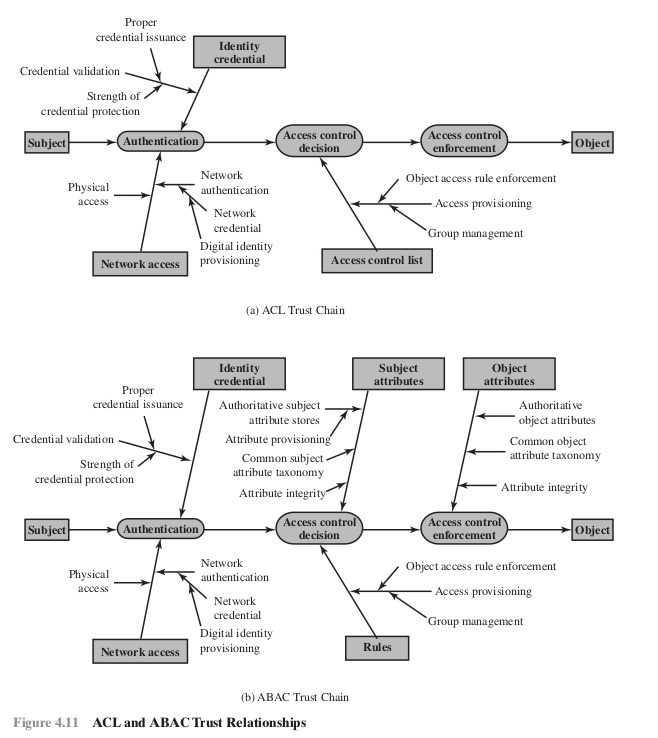
\includegraphics[width=12cm, keepaspectratio]{Bistarelli/img/cap_4/figura4.11.png}
\end{figure}

ATTR(s), ATTR(o), e ATTR(e) sono relazioni di assegnazione di attributi per il soggetto s, oggetto o, e ambiente e, rispettivamente:

\begin{figure}[H]
	\centering
    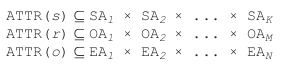
\includegraphics[width=10cm, keepaspectratio]{Bistarelli/img/cap_4/figura4.png}
\end{figure}

Usiamo anche la notazione di funzione per l'assegnazione del valore dei singoli attributi. Per esempio:

\begin{figure}[H]
	\centering
    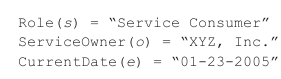
\includegraphics[width=10cm, keepaspectratio]{Bistarelli/img/cap_4/figura4-2.png}
\end{figure}

Nella forma più generale, una Policy Rule, che decide se un soggetto s può accedere ad un oggetto o in un particolare ambiente e, è una funzione booleana degli attributi di s, o ed e:
Inserire immagine

Una base di regole di policy o policy store può consistere in un certo numero di regole di policy, che coprono molti soggetti e oggetti all'interno di un dominio di sicurezza. Il controllo dell'accesso Il processo decisionale del controllo d'accesso equivale essenzialmente alla valutazione delle regole di nell'archivio delle politiche.

Ora considerate l'esempio di un negozio di intrattenimento online che trasmette film agli utenti per una tariffa mensile fissa. Useremo questo esempio per contrastare gli approcci RBAC e ABAC approcci. Il negozio deve applicare la seguente politica di controllo degli accessi basata sull'età all'età dell'utente e alla classificazione del contenuto del film:

\begin{figure}[H]
	\centering
    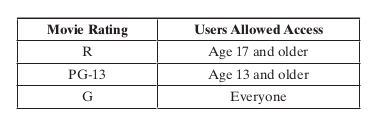
\includegraphics[width=10cm, keepaspectratio]{Bistarelli/img/cap_4/tabella4.png}
\end{figure}

In un modello RBAC, ad ogni utente verrebbe assegnato uno dei tre ruoli: Adulto, Juvenile, o Child, possibilmente durante la registrazione. Ci sarebbero tre permessi creati: Può vedere film vietati ai minori, Può vedere film vietati ai minori, e Può vedere i film vietati ai minori. Il ruolo Adulto viene assegnato con tutti e tre i permessi.

Il ruolo Juvenile ottiene le autorizzazioni Can view PG-13-rated movies e Can view G-rated movies e il ruolo Bambino ottiene solo il permesso di visualizzare i film vietati ai minori.

Entrambe le assegnazioni utente-ruolo e permesso-ruolo sono compiti amministrativi manuali. L'approccio ABAC a questa applicazione non ha bisogno di definire esplicitamente i ruoli. Invece, se un utente u può accedere o vedere un film m (in un ambiente di sicurezza e che qui viene ignorato) verrebbe risolto valutando una regola di policy come la seguente:

\begin{figure}[H]
	\centering
    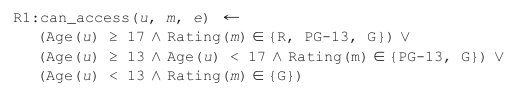
\includegraphics[width=11cm, keepaspectratio]{Bistarelli/img/cap_4/formula.png}
\end{figure}

dove Age e Rating sono rispettivamente l'attributo soggetto e l'attributo oggetto. Il vantaggio del modello ABAC mostrato qui è che elimina la definizione e la gestione di ruoli statici, eliminando così la necessità di compiti amministrativi per l'assegnazione da utente a ruolo e da permesso a ruolo.

Il vantaggio di ABAC si vede più chiaramente quando imponiamo politiche a grana più fine. Per esempio, supponiamo che i film siano classificati come New Release o Old Release, in base alla data di rilascio rispetto alla data corrente, e che gli utenti siano classificati come classificati come Utente Premium e Utente Regolare, in base alla tariffa che pagano. Vorremmo applicare una politica per cui solo gli utenti premium possono vedere i nuovi film. Per il modello RBAC, dovremmo raddoppiare il numero di ruoli, per distinguere ogni utente per età e tariffa, e dovremmo raddoppiare il numero di permessi separati pure.

In generale, se ci sono K attributi soggetto e M attributi oggetto, e se per ogni attributo, Range() denota l'intervallo di valori possibili che può assumere, allora il rispettivo numero di ruoli e permessi richiesti per un modello RBAC sono:

\begin{figure}[H]
	\centering
    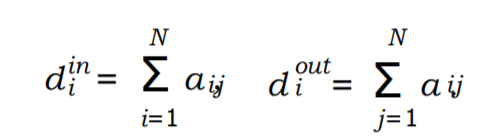
\includegraphics[width=11cm, keepaspectratio]{Bistarelli/img/cap_4/formula2.png}
\end{figure}

Così, possiamo vedere che quando il numero di attributi aumenta per ospitare politiche a grana più fine, il numero di ruoli e permessi cresce esponenzialmente.

Al contrario, il modello ABAC tratta gli attributi aggiuntivi in modo efficiente. Per questo esempio, la policy R1 definita in precedenza è ancora valida. Abbiamo bisogno di due nuove regole:

\begin{figure}[H]
	\centering
    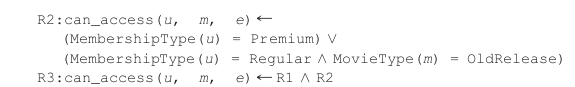
\includegraphics[width=12cm, keepaspectratio]{Bistarelli/img/cap_4/foto4-3.png}
\end{figure}

Con il modello ABAC, è anche facile aggiungere attributi ambientali. Supponiamo che che vogliamo aggiungere una nuova regola di policy che è espressa in parole come segue: Gli utenti regolari sono autorizzati a vedere le nuove release nei periodi promozionali. Questo sarebbe difficile da esprimere in un modello RBAC. In un modello ABAC, abbiamo solo bisogno di aggiungere una regola congiuntiva (AND) che controlla per vedere se l'attributo ambientale la data di oggi cade in un periodo promozionale.
\newpage
\section{Gestione dell'entità, delle credenziali e dell'accesso}
L'ICAM è un approccio completo alla gestione e all'implementazione delle identità digitali identità digitali (e gli attributi associati), le credenziali e il controllo degli accessi. ICAM è stato sviluppato dal governo degli Stati Uniti, ma è applicabile non solo alle agenzie governative, ma può anche essere distribuito da imprese che cercano un approccio unificato al controllo degli accessi. ICAM è progettato per:
\begin{itemize}

    \item Creare rappresentazioni fidate di identità digitali di individui e di ciò che i documenti ICAM si riferiscono a entità non personali (NPE). Queste ultime includono processi, applicazioni e dispositivi automatici che cercano di accedere a una risorsa.
    
    \item Legare queste identità a credenziali che possono servire come proxy per l'individuo o NPE nelle transazioni di accesso. Una credenziale è un oggetto o una struttura di dati che lega autorevolmente un'identità (e opzionalmente, attributi aggiuntivi) a un token posseduto e controllato da un sottoscrittore.
    
    \item Utilizza le credenziali per fornire un accesso autorizzato alle risorse di un'agenzia.
\end{itemize}
\newpage
\subsection{Gestione dell'identità}
La gestione dell'identità si occupa di assegnare attributi a un'identità digitale e di collegare tale identità digitale a un individuo o a una NPE. L'obiettivo è quello di stabilire un'identità digitale affidabile che sia indipendente da una specifica applicazione o contesto.

\singlespacing

L'approccio tradizionale, e ancora più comune, al controllo dell'accesso per applicazioni e programmi è quello di creare una rappresentazione digitale di un'identità per l'uso specifico di l'applicazione o il programma. Di conseguenza, il mantenimento e la protezione dell'identità stessa è trattata come secondaria rispetto alla missione associata all'applicazione. Inoltre, c'è una considerevole sovrapposizione di sforzi nello stabilire queste identità specifiche dell'applicazione.

\singlespacing

A differenza degli account usati per accedere a reti, sistemi o applicazioni, i record di identità aziendali non sono legati al titolo di lavoro, alle mansioni lavorative, all'ubicazione o al fatto che sia necessario l'accesso a un sistema specifico. Questi elementi possono diventare attributi legati ad un record di identità e possono anche diventare parte di ciò che identifica in modo univoco un individuo in una specifica applicazione. Le decisioni sul controllo degli accessi saranno basate sul contesto e sugli attributi rilevanti di un utente non solo sulla sua identità. Il concetto di un'identità aziendale è che gli individui avranno una singola rappresentazione digitale di se stessi che può essere sfruttata in tutti i dipartimenti e le agenzie per molteplici scopi, compreso il controllo degli accessi.

\singlespacing

\begin{figure}[H]
	\centering
    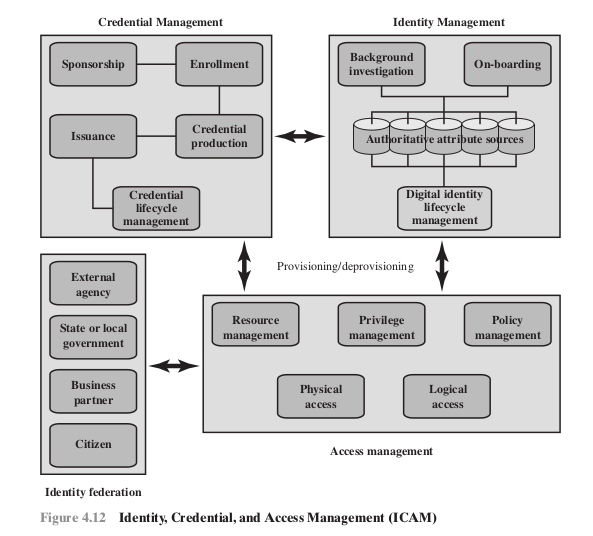
\includegraphics[width=10cm, keepaspectratio]{Bistarelli/img/cap_4/figura4.12.png}
\end{figure}

La figura 4.12 illustra le funzioni chiave coinvolte nella gestione delle identità. Un'identità digitale inizia tipicamente con la raccolta di dati di identità come parte di un processo di iscrizione. Un'identità digitale è spesso composta da un insieme di attributi che aggregati identificano in modo univoco un utente all'interno di un sistema o di un'azienda. Al fine di stabilire la fiducia nell'individuo rappresentato da un'identità digitale, un'agenzia può anche condurre un'indagine di fondo.

\singlespacing

Gli attributi di un individuo possono essere memorizzati in varie fonti autorevoli all'interno di un'agenzia e collegati per formare una visione aziendale dell'identità digitale. Questa identità digitale può quindi essere fornita in applicazioni per supportare l'accesso fisico e logico (parte della gestione degli accessi) e de-provisionata quando l'accesso non è più richiesto.

\singlespacing

Un elemento finale della gestione delle identità è la gestione del ciclo di vita, include quanto segue:

\begin{itemize}
    \item Meccanismi, politiche e procedure per proteggere l'identità personale informazioni
    
    \item Controllo dell'accesso ai dati di identità
    
    \item Tecniche per condividere dati di identità autorevoli con le applicazioni che ne hanno bisogno

    \item Revoca di un'identità aziendale
\end{itemize}
\newpage
\subsection{Gestione delle credenziali}
Come detto, una credenziale è un oggetto o una struttura di dati che lega autorevolmente un'identità (e opzionalmente, attributi aggiuntivi) ad un token posseduto e controllato da un sottoscrittore. Esempi di credenziali sono le smart card, le chiavi crittografiche private/pubbliche crittografiche private/pubbliche e i certificati digitali. La gestione delle credenziali è la gestione del ciclo di vita ciclo di vita della credenziale.
\singlespacing
La gestione delle credenziali comprende i seguenti cinque componenti logistici:
\begin{enumerate}
    \item Un individuo autorizzato sponsorizza un individuo o un'entità per una credenziale per stabilire la necessità della credenziale. Per esempio, un supervisore di reparto sponsorizza un dipendente del dipartimento.

    \item L'individuo sponsorizzato si iscrive per la credenziale, un processo che tipicamente consiste in una prova d'identità e nella cattura di dati biografici e di dati di sicurezza.

un processo che tipicamente consiste nella prova dell'identità e nell'acquisizione di dati biografici e biometrici. Questo passo può anche comportare l'incorporazione di dati di attributo autorevoli, mantenuti dal dal componente di gestione dell'identità.

    \item Viene prodotta una credenziale. A seconda del tipo di credenziale, la produzione può coinvolgere la crittografia, l'uso di una firma digitale, la produzione di una smartcard, o altre funzioni.

    \item La credenziale viene rilasciata all'individuo o alla NPE.
    
    \item Una credenziale deve essere mantenuta durante il suo ciclo di vita, che potrebbe includere la revoca, la riemissione/sostituzione, la reiscrizione, la scadenza, la reimpostazione del numero di identificazione personale (PIN), sospensione o reintegrazione.
\end{enumerate}
\newpage
\subsection{Gestione degli accessi}
Il componente di gestione degli accessi si occupa della gestione e del controllo delle modalità di accesso alle risorse da parte delle entità. Copre sia l'accesso logico che fisiologico e può essere interno ad un sistema o un elemento esterno. Lo scopo della gestione degli accessi è quello di garantire che venga fatta la corretta verifica dell'identità quando un individuo tenta di accedere a edifici, sistemi informatici o dati sensibili alla sicurezza. La funzione di controllo degli accessi fa uso delle credenziali presentate da chi richiede l'accesso e l'identità digitale del richiedente.
\singlespacing
Sono necessari tre elementi di supporto per una struttura di controllo degli accessi a livello aziendale:
\begin{itemize}
    \item \textbf{Gestione delle risorse}
    
Questo elemento riguarda la definizione di regole per una risorsa che richiede il controllo dell'accesso. Le regole includeranno le credenziali requisiti delle credenziali e quali attributi dell'utente, attributi della risorsa e condizioni ambientali sono richieste per l'accesso ad una data risorsa per una data funzione.

\item \textbf{Gestione dei privilegi}

Questo elemento si occupa di stabilire e mantenere di diritti o attributi di privilegio che comprendono il profilo di accesso di un individuo. Questi attributi rappresentano caratteristiche di un individuo che possono essere utilizzati come base per determinare le decisioni di accesso alle risorse fisiche e logiche. I privilegi sono considerati attributi che possono essere collegati a un'identità digitale. identità digitale.

\item \textbf{Gestione delle politiche}

Questo elemento governa ciò che è permesso e non permesso in una transazione di accesso. Cioè, dati l'identità e gli attributi del richiedente, gli attributi della risorsa o dell'oggetto e le condizioni ambientali, una politica specifica quali azioni questo utente può eseguire su questo oggetto.
\end{itemize}
\newpage
\subsection{Federazione delle identità}
La federazione di identità affronta due questioni:
\begin{enumerate}
    \item Come vi fidate delle identità di individui di organizzazioni esterne che hanno bisogno di accesso ai vostri sistemi?
    
    \item Come garantisci le identità degli individui della tua organizzazione quando hanno hanno bisogno di collaborare con organizzazioni esterne?
\end{enumerate}
La federazione delle identità è un termine usato per descrivere la tecnologia, gli standard, le politiche e processi che permettono a un'organizzazione di fidarsi di identità digitali, attributi di identità e credenziali create ed emesse da un'altra organizzazione.
\section{Strutte di fiducia}
I concetti interconnessi di fiducia, identità e attributi sono diventati preoccupazioni fondamentali delle imprese Internet, dei fornitori di servizi di rete e delle grandi imprese. Queste preoccupazioni possono essere viste chiaramente nell'ambiente del commercio elettronico. Per l'efficienza, la privacy e la semplicità legale, le parti delle transazioni generalmente applicano il principio del need-to-know: cosa si deve sapere di qualcuno per trattare con lui? La risposta varia da caso a caso, e include attributi come il numero di registrazione professionale o di licenza, l'organizzazione e il dipartimento, l'ID del personale, il nulla osta di sicurezza, il numero di riferimento del cliente, il numero di carta di credito, l'identificatore unico della salute, le allergie, il gruppo sanguigno, il numero di previdenza sociale, l'indirizzo, lo stato di cittadino, il nickname dei social network, lo pseudonimo e così via. Gli attributi di un individuo che devono essere conosciuti e verificati per permettere una transazione dipendono dal contesto. Per esempio, un'impresa può bisogno di fornire accesso alle risorse per clienti, utenti, fornitori e partner. A seconda del contesto, l'accesso sarà determinato non solo dall'identità, ma dagli attributi del richiedente e della risorsa.
\newpage
\subsection{Approccio tradizionale allo scambio di identità}
Le transazioni online o in rete che coinvolgono parti di diverse organizzazioni, o tra un'organizzazione e un utente individuale come un cliente online, richiedono generalmente la condivisione di informazioni di identità. Queste informazioni possono includere una serie di attributi associati oltre a un semplice nome o identificatore numerico. Sia la parte che divulga le informazioni che quella che le riceve devono avere un livello di fiducia sulle questioni di sicurezza e di privacy relative a tali informazioni. La figura 4.13a mostra la tecnica tradizionale per lo scambio di informazioni sull'identità. Questo comporta che gli utenti sviluppino accordi con un fornitore di servizi di identità per procurarsi identità e credenziali digitali, e accordi con le parti che forniscono servizi e applicazioni per gli utenti finali e che sono disposti a fare affidamento sull'identità e sulle informazioni sull'identità e le credenziali generate dal fornitore di servizi d'identità. L'accordo della Figura 4.13a deve soddisfare una serie di requisiti. La parte fidata richiede che l'utente sia stato autenticato con un certo grado di sicurezza, che gli attributi imputati all'utente dal fornitore di servizi d'identità siano accurati, e che il fornitore di servizi d'identità sia autorevole per quegli attributi. Il fornitore di servizi d'identità richiede l'assicurazione di avere informazioni accurate sull'utente e che, se condivide le informazioni, la parte che si affida le userà in accordo con i termini e le condizioni contrattuali e la legge. L'utente richiede l'assicurazione che al fornitore di servizi d'identità e alla parte fidata possano essere affidate informazioni sensibili e che si attengano alle preferenze dell'utente e rispettino la sua privacy. Soprattutto, tutte le parti vogliono sapere se le pratiche descritte dalle altre parti sono effettivamente quelle attuate dalle parti, e quanto sono affidabili quelle parti.
\subsection{Approccio di fiducia per l'identità aperta}

\begin{figure}[H]
	\centering
    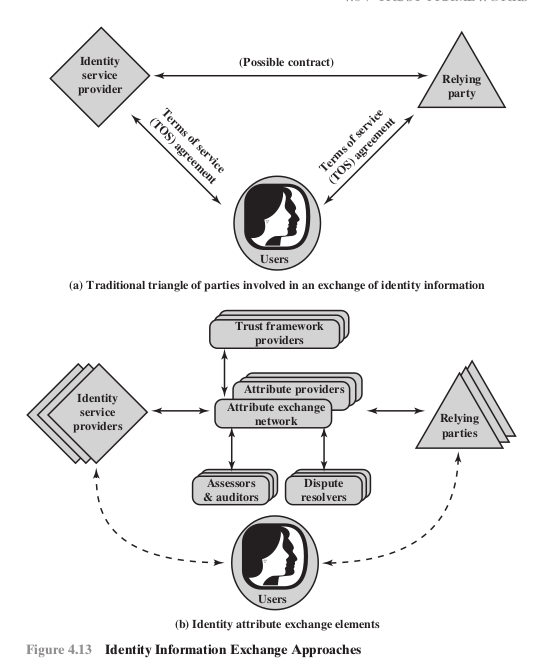
\includegraphics[width=10cm, keepaspectratio]{Bistarelli/img/cap_4/figura4.13.png}
\end{figure}


Senza qualche standard e quadro universale, la disposizione della Figura 4.13a deve essere replicata in molteplici contesti. Un approccio di gran lunga preferibile è quello di sviluppare un approccio aperto e standardizzato per lo scambio di identità e attributi affidabili. Nel resto di questa sezione, esaminiamo un tale approccio che sta guadagnando sempre più consenso. Sfortunatamente, questo argomento è gravato da numerosi acronimi, quindi è meglio iniziare con una definizione del più importante di questi:
\begin{itemize}
    \item \textbf{OpenId}
    
    Questo è uno standard aperto che permette agli utenti di essere autenticati da alcuni siti cooperanti (noti come Relying Parties) utilizzando un servizio di terze parti, eliminando la necessità per i webmaster di fornire i propri sistemi ad hoc e permettendo agli utenti di consolidare le loro identità digitali. Gli utenti possono creare account con i loro fornitori di identità OpenID preferiti, quindi utilizzare tali account come base per accedere a qualsiasi sito web che accetti l'autenticazione OpenID.
    
    \item \textbf{OIDF}
    
    La OpenID Foundation è un'organizzazione internazionale senza scopo di lucro di persone e aziende impegnate ad abilitare, promuovere e proteggere le tecnologie OpenID. OIDF assiste la comunità fornendo l'infrastruttura necessaria struttura e aiuto nel promuovere e sostenere l'adozione estesa di OpenID.
    
    \item \textbf{ICF}
    
    La Information Card Foundation è una comunità senza scopo di lucro di aziende e individui che lavorano insieme per far evolvere l'ecosistema Information Card. Le carte d'informazione sono identità digitali personali che le persone possono usare online, e la componente chiave dei metasistemi di identità. Visivamente, ogni Information Card ha un'immagine a forma di carta e un nome di carta associato ad essa che permette alle persone di organizzare le loro identità digitali e di selezionare facilmente quella che vogliono usare per qualsiasi interazione.
    
    \item \textbf{OITF}
    
    La Information Card Foundation è una comunità senza scopo di lucro di aziende e individui che lavorano insieme per far evolvere l'ecosistema Information Card. Le carte d'informazione sono identità digitali personali che le persone possono usare online, e la componente chiave dei metasistemi di identità. Visivamente, ogni Information Card ha un'immagine a forma di carta e un nome di carta associato ad essa che permette alle persone di organizzare le loro identità digitali e di selezionare facilmente quella che vogliono usare per qualsiasi interazione.
    
    \item \textbf{OIX}
    
    L'Open Identity Exchange Corporation è un fornitore internazionale indipendente e neutrale internazionale di strutture di fiducia per la certificazione conformi al modello Open Identity Trust Frameworks.
    
    \item \textbf{AXN}
    
    Un Attribute Exchange Network (AXN) è un gateway online su scala Internet per i fornitori di servizi d'identità e per le parti che si affidano a loro per accedere in modo efficiente agli attributi di identità online affermati dall'utente, autorizzati e verificati in volumi a costi accessibili.

    
\end{itemize}
I gestori del sistema devono potersi fidare del fatto che gli attributi associati a un soggetto o un oggetto siano autorevoli e vengano scambiati in modo sicuro. Un approccio per fornire tale fiducia all'interno di un'organizzazione è il modello ICAM, in particolare i componenti ICAM (vedi figura 4.12). Combinato con una funzionalità di federazione di identità che è condivisa con altre organizzazioni, gli attributi possono essere scambiati in modo degno di fiducia, supportando un controllo di accesso sicuro. Nei sistemi d'identità digitale, una struttura di fiducia funziona come un programma di certificazione. Permette ad una parte che accetta una credenziale di identità digitale (chiamata parte fidata) di fidarsi delle politiche di identità, sicurezza e privacy della parte che emette la credenziale (chiamato fornitore di servizi di identità) e viceversa.
\singlespacing
Più formalmente, OIX definisce un quadro di fiducia come un insieme di impegni verificabili da ciascuna delle varie parti di una transazione verso le loro controparti.
\singlespacing
Questi impegni includono:
\begin{enumerate}
    \item Controlli (compresi gli obblighi normativi e contrattuali) per aiutare a garantire che gli impegni siano
    
    \item Rimedi per il mancato rispetto di tali impegni.
\end{enumerate}
Un quadro di fiducia è sviluppato da una comunità i cui membri hanno obiettivi e prospettive simili. Esso definisce i diritti e le responsabilità dei partecipanti di quella comunità; specifica le politiche e gli standard specifici della comunità e definisce i processi e le processi e procedure specifiche della comunità che forniscono garanzie. Possono esistere diversi quadri di fiducia, e i gruppi di partecipanti possono personalizzare le strutture di fiducia per soddisfare le loro particolari esigenze. La figura 4.13b mostra gli elementi coinvolti nell'OITF.
\singlespacing
All'interno di una data organizzazione o agenzia, i seguenti ruoli sono parte del quadro generale:
\begin{itemize}
    \item \textbf{Relying parties (RPs):} Chiamati anche fornitori di servizi, sono entità che forniscono servizi a specifici utenti. Le RP devono avere fiducia nelle identità e/o negli attributi dei loro utenti, e devono fare affidamento sulle varie credenziali presentate per dimostrare tali attributi e identità.

    \item \textbf{Soggetti:} Questi sono gli utenti dei servizi di una RP, compresi i clienti, gli impiegati, partner commerciali e abbonati.

    \item \textbf{Fornitori di attributi (AP):} Gli AP sono entità riconosciute dalla comunità di interesse come in grado di verificare determinati attributi come presentati dai soggetti e che sono attrezzati attraverso l'AXN per creare credenziali di attributo conformi secondo le regole e gli accordi dell'AXN. Alcuni AP saranno fonti di autorità per certe informazioni; più comunemente gli AP saranno broker di attributi derivati.

    \item \textbf{Fornitori di identità (IDP):} Queste sono entità in grado di autenticare le credenziali degli utenti e di garantire i nomi (o pseudonimi o handle) dei soggetti, e che sono attrezzati attraverso l'AXN o qualche altro sistema compatibile di Identità e (IDAM) compatibile per creare identità digitali che possono essere utilizzate per indicizzare gli attributi degli utenti.
\end{itemize}
Ci sono anche i seguenti importanti elementi di supporto come parte di un AXN:
\begin{itemize}
    \item \textbf{Valutatori:} I valutatori valutano i fornitori di servizi di identità e gli RP e certificano che sono in grado di seguire il progetto del fornitore OITF.
    
    \item \textbf{Revisori:} Queste entità possono essere chiamate a controllare che le pratiche delle parti siano state in linea con quanto concordato per l'OITF.
    
    \item \textbf{Risolutori di controversie:} Queste entità forniscono arbitrato e risoluzione delle controversie secondo le linee guida dell'OIX.
    
    \item \textbf{Fornitori di strutture di fiducia:} Un fornitore di strutture di fiducia è un'organizzazione che traduce i requisiti dei politici in un proprio progetto per una struttura di fiducia quadro di fiducia che poi procede a costruire, facendolo in un modo che è coerente con i requisiti minimi stabiliti nella specifica OITF.
\end{itemize}
In quasi tutti i casi, ci sarà un'organizzazione candidata ragionevolmente ovvia ad assumere questo ruolo, per ogni settore industriale o grande organizzazione che decide che è appropriato interoperare con un AXN.

\singlespacing

Le linee solide con le frecce nella Figura 4.13b indicano gli accordi con il fornitore del quadro fiduciario per l'implementazione dei requisiti tecnici, operativi e legali. Le linee tratteggiate indicano altri accordi potenzialmente interessati da questi requisiti. In termini generali, il modello illustrato nella Figura 4.13b funzionerebbe nel modo seguente. Le persone responsabili all'interno delle organizzazioni partecipanti determinano i requisiti tecnici, operativi e legali per gli scambi di informazioni sull'identità che ricadono sotto la loro autorità. Quindi selezionano i fornitori dell'OITF per implementare questi requisiti. Questi fornitori dell'OITF traducono i requisiti in un progetto per un quadro di fiducia che può includere ulteriori condizioni del fornitore dell'OITF. Il fornitore dell'OITF esamina i fornitori di servizi d'identità e gli RP e stipula con loro dei contratti per seguire i requisiti del suo quadro di fiducia quando conduce scambi di informazioni sull'identità. I contratti contengono disposizioni relative ai risolutori di controversie e ai revisori per l'interpretazione e l'applicazione del contratto.
\newpage
\section{Caso di studio: Sistema RBAC per una banca}
La Dresdner Bank ha implementato un sistema RBAC che serve come utile esempio pratico.
\paragraph{Esempio pratico} La banca usa una varietà di applicazioni informatiche. Molte di queste sono state inizialmente sviluppate per un ambiente mainframe; alcune di queste vecchie applicazioni sono ora supportate su una rete client-server, mentre altre rimangono su mainframe. Ci sono anche applicazioni più recenti su server. Prima del 1990, un semplice sistema DAC era usato su ogni server e mainframe. Gli amministratori mantenevano un file di controllo dell'accesso locale su ogni host e definivano i diritti di accesso per ogni dipendente su ogni applicazione su ogni host. Questo sistema era ingombrante, dispendioso in termini di tempo e soggetto a errori. Per migliorare il sistema, la banca ha introdotto uno schema RBAC, che è a livello di sistema e in cui la determinazione dei diritti di accesso è compartimentata in tre diverse unità amministrative per una maggiore sicurezza. I ruoli all'interno dell'organizzazione sono definiti da una combinazione di posizione ufficiale e funzione lavorativa. La tabella 4.5a fornisce degli esempi. Questo differisce un po' dal concetto di ruolo nello standard NIST, in cui un ruolo è definito da una funzione lavorativa. In una certa misura, la differenza è una questione di terminologia. In ogni caso, la strutturazione dei ruoli della banca porta a un mezzo naturale per sviluppare una gerarchia di eredità basata sulla posizione ufficiale. All'interno della banca, c'è un rigido ordine parziale delle posizioni ufficiali all'interno di ogni organizzazione, che riflette una gerarchia di responsabilità e potere. Per esempio, le posizioni di capo divisione, direttore di gruppo e impiegato sono in ordine decrescente. Quando la posizione ufficiale è combinata con la funzione lavorativa, c'è un conseguente un ordinamento dei diritti di accesso, come indicato nella tabella 4.5b. Così, l'analista finanziario/Group Manager (ruolo B) ha più diritti di accesso rispetto al ruolo analista finanziario/commesso (ruolo A). La tabella indica che il ruolo B ha altrettanti o più diritti di accesso del ruolo A in tre applicazioni e ha diritti di accesso a una quarta applicazione. D'altra parte, non c'è una relazione gerarchica tra office banking/Group Manager e l'analista finanziario/commesso perché lavorano in aree funzionali diverse. Possiamo definire una gerarchia di ruoli in cui un ruolo è superiore ad un altro se la sua posizione è superiore e le loro funzioni sono identiche. La gerarchia dei ruoli permette di risparmiare sulle definizioni dei diritti di accesso, come suggerito nella tabella 4.5c.

\singlespacing

\begin{figure}[H]
	\centering
    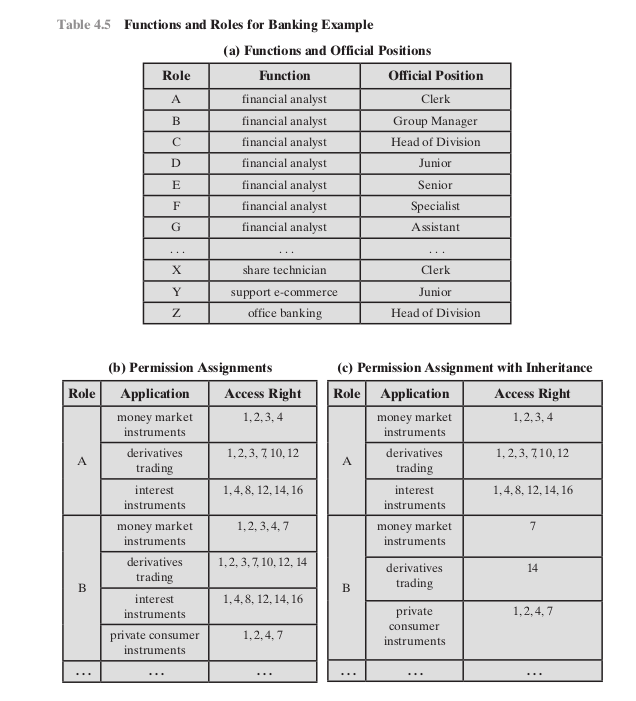
\includegraphics[width=12cm, keepaspectratio]{Bistarelli/img/cap_4/tabella4.5.png}
\end{figure}

Nello schema originale, l'assegnazione diretta dei diritti di accesso al singolo utente avveniva a livello di applicazione ed era associata alla singola applicazione. Nel nuovo schema, un'amministrazione dell'applicazione determina l'insieme dei diritti di accesso associati ad ogni singola applicazione. Tuttavia, un dato utente che esegue un dato compito potrebbe non avere tutti i diritti di accesso associati all'applicazione. applicazione. Quando un utente invoca un'applicazione, l'applicazione concede l'accesso sulla sulla base di un profilo di sicurezza fornito a livello centrale. Un'amministrazione separata delle autorizzazioni associa i diritti di accesso ai ruoli e crea il profilo di sicurezza per un uso sulla sulla base del ruolo dell'utente. Ad un utente viene assegnato staticamente un ruolo. In linea di principio (in questo esempio), ogni utente può essere assegnato staticamente fino a quattro ruoli e selezionare un dato ruolo da usare per invocare una particolare applicazione. Questo corrisponde al concetto NIST di sessione. In pratica, la maggior parte utenti sono assegnati staticamente a un singolo ruolo in base alla posizione dell'utente e alla sua funzione lavorativa. Tutti questi ingredienti sono rappresentati nella Figura 4.14. Il Dipartimento Risorse Umane assegna un ID utente unico ad ogni dipendente che userà il sistema.

\singlespacing

\begin{figure}[H]
	\centering
    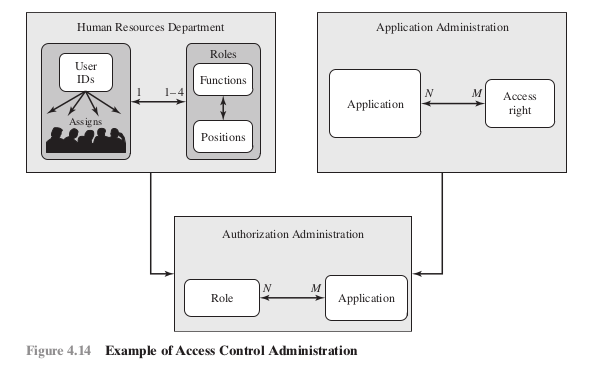
\includegraphics[width=12cm, keepaspectratio]{Bistarelli/img/cap_4/figura4.14.png}
\end{figure}

In base alla posizione e alla funzione lavorativa dell'utente, il dipartimento assegna anche uno o ruoli all'utente. Le informazioni sull'utente/ruolo sono fornite all'Amministrazione delle autorizzazioni Amministrazione, che crea un profilo di sicurezza per ogni utente che associa l' ID utente e il ruolo a un insieme di diritti di accesso. Quando un utente invoca un'applicazione, l'applicazione consulta il profilo di sicurezza per quell'utente per determinare quale sottoinsieme dei diritti di accesso dell'applicazione sono in vigore per questo utente in questo ruolo. Un ruolo può essere usato per accedere a diverse applicazioni. Così, l'insieme dei diritti di accesso associati a un ruolo possono includere diritti di accesso che non sono associati a una delle applicazioni che l'utente invoca. Questo è illustrato nella tabella 4.5b. Il ruolo A ha numerosi diritti di accesso, ma solo un sottoinsieme di questi diritti è applicabile a ciascuna delle tre applicazioni che il ruolo A può invocare.

\singlespacing

Alcune cifre su questo sistema sono interessanti. All'interno della banca, ci sono 65 posizioni ufficiali, che vanno da un impiegato in una filiale, attraverso il direttore di filiale, a un membro del consiglio di amministrazione. Queste posizioni sono combinate con 368 diverse funzioni lavorative fornite dal database delle risorse umane. Potenzialmente, ci sono 23.920 ruoli diversi, ma il numero di ruoli attualmente in uso è di circa 1.300. Questo è in linea con l'esperienza di altre implementazioni RBAC. In media, 42.000 profili di sicurezza sono distribuiti alle applicazioni ogni giorno dal modulo di amministrazione delle autorizzazioni.














